\documentclass[12pt]{article}

\usepackage{graphicx,url}
\usepackage[utf8]{inputenc}
\usepackage{bm}
\usepackage{amsmath}
\usepackage{amssymb}
\usepackage{systeme}
\usepackage{chngcntr}

\usepackage{fancyhdr}
\usepackage{extramarks}
\usepackage{amsmath}
\usepackage{amsthm}
\usepackage{amsfonts}
\usepackage{tikz}
\usepackage[plain]{algorithm}
\usepackage{algpseudocode}
\usepackage{chngcntr}
\usepackage{tikz}
\usepackage{color}

\usetikzlibrary{automata,positioning}

%
% Basic Document Settings
%

\topmargin=-0.45in
\evensidemargin=0in
\oddsidemargin=0in
\textwidth=6.5in
\textheight=9.0in
\headsep=0.25in
\linespread{1.1}

\counterwithin*{equation}{section}
\counterwithin*{equation}{subsection}
\newcommand{\sol} {\textbf{Solution:}}
\newcommand{\A} {\mathbf{A}}
\newcommand{\B} {\mathbf{B}}
\newcommand{\C} {\mathbf{C}}
\newcommand{\RREF} {Reduced Row-Echelon Form}
\newcommand{\REMM} {Row-Equivalent Matrices}
\newcommand{\pivot} {$\boxed{1}$~}
\newcommand{\ls} {\(\mathcal{LS}(A,\textbf{0})\)}
\newcommand{\nullspace}[1]{\mathcal{N}(#1)}
\newcommand{\p} {$\boxed{1}$~}
\newcommand*\Domain[1]{\in\mathbb{C}^{#1}}

\newcommand{\matx}[1] {
\begin{bmatrix}
  #1 \\
\end{bmatrix}
}

\newcommand{\matxx}[2] {
\begin{bmatrix}
  #1 \\
  #2 \\
\end{bmatrix}
}

\newcommand{\matxxx}[3] {
\begin{bmatrix}
  #1 \\
  #2 \\
  #3 \\
\end{bmatrix}
}

\newcommand{\matxxxx}[4] {
\begin{bmatrix}
  #1 \\
  #2 \\
  #3 \\
  #4 \\
\end{bmatrix}
}
\newcommand{\matxxxxx}[5] {
\begin{bmatrix}
  #1 \\
  #2 \\
  #3 \\
  #4 \\
  #5 \\
\end{bmatrix}
}

\newcommand{\matxxxxxx}[6] {
\begin{bmatrix}
  #1 \\
  #2 \\
  #3 \\
  #4 \\
  #5 \\
  #6 \\
\end{bmatrix}
}

\newcommand{\arrow}[1] {\xrightarrow[]{\text{#1}}}

\title{Project 1}
\date{Linear Algebra}

\author{Yong Hoon Do, Dongwook Kim, Chanyang Yim}

\begin{document}

\maketitle

%--------------------------------------------------------------------------------
\section{\bigskip\vspace{0in}\vspace{-0.1in}Exercise 1}

\noindent\textbf{Exercise 1.1} Set up a system of linear equations based on
this problem from the \textit{Nine Chapters on the Mathematical Art}.

\bigskip

The text then shows three columns set up on a counting board (a tool for
mathematical calculation) in the following manner:

\bigskip

The given augmented matrix is:

\[
  \begin{array}{cccc}
    1 & 2 & 3 \\
    2 & 3 & 2 \\
    3 & 1 & 1 \\
    26 & 34 & 39 \\
  \end{array}
\]

\sol

Setting the system of linear equations:

\begin{equation}
  \begin{array}{cccc}
    3x_1 + 2x_2 + x_3 = 39 \\
    2x_1 + 3x_2 + x_3 = 34 \\
    x_1 + 2x_2 + 3x_3 = 26 \\
  \end{array}
\end{equation}

\bigskip

%--------------------------------------------------------------------------------
\bigskip\noindent\textbf{Exercise 1.2} Write the equations you found in
Exercise 1.1 as an augmented matrix. How does your matrix compare with the
numbers on the counting board?

\sol

Setting the augmented matrix found in the \bigskip\noindent\textbf{Exercise 1.1}:
\[
\left|
  \begin{array}{cccc}
    3 & 2 & 1 & 39 \\
    2 & 3 & 1 & 34 \\
    1 & 2 & 3 & 26 \\
  \end{array}
\right|
\]

The major difference between the matrices is the order how the numbers are listed. According to the book \textit{Nine Chapters on the Mathematical Art}, they vertically
listed up the variables and created a matrix in this same fashion. The way how seprating the coefficient variables is also
following their writing order; from right to left and top to bottom. As this way of writing order used during Han Dynasty,
creating matrix also followed the same method that they used for writing chiense letters.


\bigskip

%--------------------------------------------------------------------------------
\bigskip\noindent\textbf{Exercise 1.3} Use row operations to get your
augmented matrix from Exercise 1.2 into row-echelon form and solve the system
of equations.

\bigskip

\bigskip
Work to reduced row-echelon form,

first with j = $1$~,

\[
\begin{bmatrix}
    	3 & 2 & 1 & 39\\
        2 & 3 & 1 & 34 \\
        1 & 2 & 3 & 26 \\
	\end{bmatrix}
    \xrightarrow[]{\text{$R\textsubscript{1} \leftrightarrow R\textsubscript{3}$~}}
    \begin{bmatrix}
    	1 & 2 & 3 & 26 \\
        2 & 3 & 1 & 34 \\
        3 & 2 & 1 & 39\\
	\end{bmatrix}
\]

\[
    \xrightarrow[]{\text{$-2R\textsubscript{1} + R\textsubscript{2}$~}}
    \begin{bmatrix}
    	1 & 2 & 3 & 26 \\
        0 & -1 & -5 & -18 \\
        3 & 2 & 1 & 39\\
	\end{bmatrix}
\xrightarrow[]{\text{$-3R\textsubscript{1} + R\textsubscript{3}$~}}
    \begin{bmatrix}
    	1 & 2 & 3 & 26 \\
        0 & -1 & -5 & -18 \\
        0 & -4 & -8 & -39\\
	\end{bmatrix}
\]

Now, with j = 2,
\[
\xrightarrow[]{\text{$-4R\textsubscript{2} + R\textsubscript{3}$~}}
    \begin{bmatrix}
    	1 & 2 & 3 & 26 \\
        0 & -1 & -5 & -18 \\
        0 & 0 & 12 & 33\\
	\end{bmatrix}
\xrightarrow[]{\text{$2R\textsubscript{2} + R\textsubscript{1}$~}}
    \begin{bmatrix}
    	1 & 0 & -7 & -10 \\
        0 & -1 & -5 & -18 \\
        0 & 0 & 12 & 33\\
	\end{bmatrix}
\xrightarrow[]{\text{$-R\textsubscript{2}$~}}
    \begin{bmatrix}
    	1 & 0 & -7 & -10 \\
        0 & 1 & 5 & 18 \\
        0 & 0 & 12 & 33\\
	\end{bmatrix}
\]
And finally, with j = 3,
\[
\xrightarrow[]{\text{$\frac{1}{12}R\textsubscript{3} $~}}
    \begin{bmatrix}
    	1 & 0 & -7 & -10 \\
        0 & 1 & 5 & 18 \\
        0 & 0 & 1 & \frac{11}{4}\\
	\end{bmatrix}
\xrightarrow[]{\text{$-5R\textsubscript{3} + R\textsubscript{2}$~}}
    \begin{bmatrix}
    	1 & 0 & -7 & -10 \\
        0 & 1 & 0 & \frac{17}{4} \\
        0 & 0 & 1 & \frac{11}{4}\\
	\end{bmatrix}
\xrightarrow[]{\text{$7R\textsubscript{3} + R\textsubscript{1}$~}}
    \begin{bmatrix}
    	\pivot & 0 & 0 & \frac{37}{4} \\
      0 & \pivot & 0 & \frac{17}{4} \\
      0 & 0 & \pivot & \frac{11}{4}\\
	\end{bmatrix}
\]

\bigskip
Thus,
\[
\begin{bmatrix}
    	1 & 0 & 0 & \frac{37}{4} \\
        0 & 1 & 0 & \frac{17}{4} \\
        0 & 0 & 1 & \frac{11}{4}\\
	\end{bmatrix}
\]

Therefore, this system of equation is:
\[x_1 = \frac{37}{4} = 9.25\]
\[x_2 = \frac{17}{4} = 4.25\]
\[x_3 = \frac{11}{4} = 2.75\]

\bigskip
%--------------------------------------------------------------------------------
\noindent\textbf{Exercise 1.4} Notice that the methods used in the
\textit{Nine Chapters} are very similar to our modern approach to solving a
system of equations. Verify that the solution that you obtained in Exercise
1.3 is the same as the solution obtained when solving the equations given by
the columns on the counting board shown below Exercise 1.3.

\bigskip

\sol

The given first counting board found in the Exercise 1.1 is as follows,

\[
\begin{array}{ccc}
  1 & 2 & 3 \\
  2 & 3 & 2 \\
  3 & 1 & 1 \\
  26 & 34 & 39 \\
\end{array}
\]

and we will call it as \(\A\) which is written in an aumented matrix

\[
\A=
\left|
  \begin{array}{cccc}
    3 & 2 & 1 & 39 \\
    2 & 3 & 1 & 34 \\
    1 & 2 & 3 & 26 \\
  \end{array}
\right|
\]


The given second counting board found in the Exercise 1.3 is as follows,

\[
\begin{array}{ccc}
  0 & 0 & 3 \\
  0 & 5 & 2 \\
  36 & 1 & 1 \\
  99 & 24 & 39 \\
\end{array}
\]

and we will call it as \(\B\) which is written in an aumented matrix

\[
\mathbf{B}=
\left|
  \begin{array}{cccc}
    3 & 2 & 1 & 39 \\
    0 & 5 & 1 & 24 \\
    0 & 0 & 36 & 99 \\
  \end{array}
  \right|
\]

According to the definition of \REMM,
we can transform the augmented matrices \(\A\) and \(\B\) into \RREF

\[
\A=
\left|
  \begin{array}{cccc}
    3 & 2 & 1 & 39 \\
    2 & 3 & 1 & 34 \\
    1 & 2 & 3 & 26 \\
  \end{array}
\right|
\xrightarrow[]{\text{RREF}}
\left|
\begin{array}{cccc}
  	$\boxed{1}$~ & 0 & 0 & \frac{37}{4} \\
    0 & $\boxed{1}$~ & 0 & \frac{17}{4} \\
    0 & 0 & $\boxed{1}$~ & \frac{11}{4} \\
  \end{array}
\right|
\]

\[
\B=
\left|
  \begin{array}{cccc}
    3 & 2 & 1 & 39 \\
    0 & 5 & 1 & 24 \\
    0 & 0 & 36 & 99 \\
  \end{array}
\right|
\xrightarrow[]{\text{RREF}}
\left|
\begin{array}{cccc}
  	$\boxed{1}$~ & 0 & 0 & \frac{37}{4} \\
    0 & $\boxed{1}$~ & 0 & \frac{17}{4} \\
    0 & 0 & $\boxed{1}$~ & \frac{11}{4} \\
  \end{array}
\right|
\]

Thus, two matrices \(\A\) and \(\B\) are row-equivalent,
and these two augmented matrices which derived from the counting board are having the same solutions.

\bigskip

%--------------------------------------------------------------------------------
\noindent\textbf{Exercise 1.5} Translate Borrel's language into a system of
simultaneous linear equations using the variables A, B and C.

\bigskip

\begin{minipage}{0.45\textwidth}
 	\begin{center}
 	  Borrel's language
 	\end{center}
	\[
    	\begin{array}{ccccc}
		3A & 1B & 1C & [42 & 1ST\\
		1A & 4B & 1C & [32 & 2ST\\
		1A & 1B & 5C & [40 & 3ST\\
		\end{array}
    \]
    \[
    	\begin{array}{cccc}
		3A & 12B & 3C & [96 \\
		3A & 1B & 1C & [42 \\
		   & 11B & 2C & [54 \\
		\end{array}
    \]
    \[
    	\begin{array}{cccc}
		3A & 3B & 15C & [120 \\
		3A & 1B & 1C & [42 \\
		   & 2B & 14C & [78 \\
		\end{array}
    \]
    \[
    	\begin{array}{cccc}
			& 22B & 154C & [858 \\
		    & 22B & 4C & [108 \\
		   	&	 & 150C & [750 \\
		\end{array}
    \]
\end{minipage}%
\hfill
\begin{minipage}{0.45\textwidth}
	\begin{center}
    System of simultaneous linear equations
  \end{center}
    \[
    	\begin{array}{c}
		3A + 1B + 1C = 42 \\
        1A + 4B + 1C = 32 \\
        1A + 1B + 5C = 40 \\
		\end{array}
    \]
    \[
    	\begin{array}{c}
		3A + 12B + 3C = 42 \\
        3A + 1B + 1C = 42 \\
             11B + 2C = 54 \\
		\end{array}
    \]
    \[
    	\begin{array}{c}
		3A + 3B + 15C = 120 \\
        3A + 1B + 1C = 42 \\
             2B + 14C = 78 \\
		\end{array}
    \]
    \[
    	\begin{array}{c}
		22B + 154C = 858 \\
        22B + 4C = 108\\
             150C = 750 \\
		\end{array}
    \]
\end{minipage}%

\bigskip

 \noindent\textbf{Exercise 1.6} Verify that Borrel's solution is correct.
\bigskip

We can verify Borrel's solution using RREF.

\bigskip
To express matrix form from Borrel's language
\[
\begin{bmatrix}
3 & 1 & 1 & 42 \\
1 & 4 & 1 & 32 \\
1 & 1 & 5 & 40 \\
\end{bmatrix}
\]

first with j=1,

\[
\xrightarrow[]{\text{$R\textsubscript{1} \leftrightarrow  R\textsubscript{3}$~}}
    \begin{bmatrix}
		1 & 1 & 5 & 40 \\
        1 & 4 & 1 & 32 \\
        3 & 1 & 1 & 42 \\
	\end{bmatrix}
\xrightarrow[]{\text{$-R\textsubscript{1} + R\textsubscript{2}$~}}
    \begin{bmatrix}
    	1 & 1 & 5 & 40 \\
        0 & 3 & -4 & -8 \\
        3 & 1 & 1 & 42 \\
	\end{bmatrix}
\xrightarrow[]{\text{$-3R\textsubscript{1} + R\textsubscript{3}$~}}
    \begin{bmatrix}
    	1 & 1 & 5 & 40 \\
        0 & 3 & -4 & -8 \\
        0 & -2 & -14 & -78 \\
	\end{bmatrix}
\]

Now, with j = 2,
\[
\xrightarrow[]{\text{$R\textsubscript{2} \leftrightarrow -\frac{1}{2}\textsubscript{3}$~}}
    \begin{bmatrix}
    	1 & 1 & 5 & 40 \\
        0 & 1 & 7 & 39 \\
        0 & 3 & -4 & -8 \\
	\end{bmatrix}
\xrightarrow[]{\text{$-3R\textsubscript{2} + R\textsubscript{3}$~}}
	\begin{bmatrix}
    	1 & 1 & 5 & 40 \\
        0 & 1 & 7 & 39 \\
        0 & 0 & -25 & -125 \\
	\end{bmatrix}
\xrightarrow[]{\text{$-R\textsubscript{2} + R\textsubscript{1}$~}}
    \begin{bmatrix}
    	1 & 0 & -2 & 1 \\
        0 & 1 & 7 & 39 \\
        0 & 0 & -25 & -125 \\
	\end{bmatrix}
\]

And finally, with j = 3,

\[
\xrightarrow[]{\text{$-\frac{1}{25}R\textsubscript{3}$~}}
    \begin{bmatrix}
    	1 & 0 & -2 & 1 \\
        0 & 1 & 7 & 39 \\
        0 & 0 & 1 & 5 \\
	\end{bmatrix}
\xrightarrow[]{\text{$7R\textsubscript{3} + R\textsubscript{2}$~}}
    \begin{bmatrix}
    	1 & 0 & -2 & 1 \\
        0 & 1 & 0 & 4 \\
        0 & 0 & 1 & 5 \\
	\end{bmatrix}
\xrightarrow[]{\text{$2R\textsubscript{3} + R\textsubscript{1} $~}}
    \begin{bmatrix}
    	1 & 0 & 0 & 11 \\
        0 & 1 & 0 & 4 \\
        0 & 0 & 1 & 5 \\
	\end{bmatrix}
\]

Thus,
\[
  \begin{bmatrix}
    	1 & 0 & 0 & 11 \\
        0 & 1 & 0 & 4 \\
        0 & 0 & 1 & 5 \\
	\end{bmatrix}
\]

This RREF tells the system of equations,

\[A = 11\]
\[B = 4\]
\[C = 5\]

Since this system of equations and Borrel's solution are same,
Borrel's solution is correct.

\bigskip

%--------------------------------------------------------------------------------
\noindent\textbf{Exercise 2.1} Use Cauchy's definition to find the
determinants of the following:

\bigskip

\sol

According to the paper, getting a determinant based on the amtrix is

\[
\begin{bmatrix}
a & b\\
c & d
\end{bmatrix}%
\xrightarrow[]{\text{Det(A)}}
ad - cb
\]

a. $%
\begin{bmatrix}
1 & 2\\
4 & -1
\end{bmatrix}
\xrightarrow[]{\text{Det(A)}}
(1)(-1)-(4)(2) = -1-8 = -9
$

\bigskip

b. $\left[
\begin{array}
[c]{cc}%
3 & -7\\
2 & 5
\end{array}
\right]
\xrightarrow[]{\text{Det(A)}}
(3)(5)-(2)(-7)=15+14=29
$

\bigskip

c. $%
\begin{bmatrix}
-2 & 3 & 0\\
1 & 2 & -1\\
-2 & 3 & 1
\end{bmatrix}
\xrightarrow[]{\text{Det(A)}}
(2)(2)(1)+(1)(3)(0)+(-2)(3)(-1)-(2)(3)(-1)-(-2)(2)(0)-(1)(3)(1)=17
$

\bigskip

d. $%
\begin{bmatrix}
5 & 0 & 4\\
1 & 2 & -1\\
-1 & -2 & 1
\end{bmatrix}
\xrightarrow[]{\text{Det(A)}}
(5)(2)(1)+(1)(-2)(4)+(-1)(0)(-1)-(5)(-2)(-1)-(-1)(2)(4)-(1)(0)(1)=0
$

\bigskip

e. $%
\begin{bmatrix}
5 & 3 & 4\\
1 & 2 & -1\\
-2 & 3 & 1
\end{bmatrix}
\xrightarrow[]{\text{Det(A)}}
(5)(2)(1)+(1)(3)(4)+(-2)(3)(-1)-(5)(3)(-1)-(-2)(2)(4)-(1)(3)(1)=56
$

\bigskip

\noindent\textbf{Exercise 2.2} For each of the matrices in Exercise 2.1 state
whether or not it is invertible and explain why.

\bigskip

\sol

All the matrices above are invertible except \textbf{d}'s matrix.
This is because every matrix can be row-reduced,
and they are nonsingular matrices
since they are square matrices and identity matrices. However, the \textbf{d}'s
 matrix is not an invertible matrix, and we found out that this is a singular matrix.

\bigskip

a. $%
\begin{bmatrix}
1 & 2\\
4 & -1
\end{bmatrix}
\xrightarrow[]{\text{RREF}}
\begin{bmatrix}
\pivot & 0 \\
0 & \pivot
\end{bmatrix}
$

\bigskip

b. $\left[
\begin{array}
[c]{cc}%
3 & -7 \\
2 & 5
\end{array}
\right]
\xrightarrow[]{\text{RREF}}
\begin{bmatrix}
\pivot & 0 \\
0 & \pivot
\end{bmatrix}
$

\bigskip

c. $%
\begin{bmatrix}
-2 & 3 & 0\\
1 & 2 & -1\\
-2 & 3 & 1
\end{bmatrix}
\xrightarrow[]{\text{RREF}}
\begin{bmatrix}
\pivot & 0 & 0 \\
0 & \pivot & 0 \\
0 & 0 & \pivot
\end{bmatrix}
$

\bigskip

d. $%
\begin{bmatrix}
5 & 0 & 4\\
1 & 2 & -1\\
-1 & -2 & 1
\end{bmatrix}
\xrightarrow[]{\text{RREF}}
\begin{bmatrix}
\pivot & 0 & \frac{4}{5} \\
0 & \pivot & -\frac{9}{10} \\
0 & 0 & 0
\end{bmatrix}
$

\bigskip

e. $%
\begin{bmatrix}
5 & 3 & 4\\
1 & 2 & -1\\
-2 & 3 & 1
\end{bmatrix}
\xrightarrow[]{\text{RREF}}
\begin{bmatrix}
\pivot & 0 & 0 \\
0 & \pivot & 0 \\
0 & 0 & \pivot
\end{bmatrix}
$

\bigskip

In addition, determinant plays the important role for determining an invertible matrix.
Inverse of \(\A\) will be evaluated as
\[
\A=
\begin{bmatrix}
a & b\\
c & d
\end{bmatrix}
,
\A^{-1} = \frac{1}{det(A)}
\begin{bmatrix}
d & -b \\
-c & a \\
\end{bmatrix}
\]

\(\A^{-1}\) won't be defined unless det\((A)\) is nonzero.
Thus, the matrices listed above are invertible since their determinants are nonzero.

\bigskip

\noindent\textbf{Exercise 2.3 }Try to determine how many terms would be
involved in using Cauchy's method for computing the determinant for a 4x4 matrix.

\sol

\[
\begin{matrix}
  a_{11} a_{22} a_{33} a_{44} +
  a_{11} a_{23} a_{34} a_{42} +
  a_{11} a_{24} a_{32} a_{43} +
  a_{12} a_{21} a_{34} a_{43} + \\
  a_{12} a_{23} a_{31} a_{44} +
  a_{12} a_{24} a_{33} a_{41} +
  a_{13} a_{21} a_{32} a_{44} +
  a_{13} a_{22} a_{34} a_{41} + \\
  a_{13} a_{24} a_{31} a_{42} +
  a_{14} a_{21} a_{33} a_{42} +
  a_{14} a_{22} a_{31} a_{43} +
  a_{14} a_{23} a_{32} a_{41} \\
  - a_{11} a_{22} a_{34} a_{43}
  - a_{11} a_{23} a_{32} a_{44}
  - a_{11} a_{24} a_{33} a_{42}
  - a_{12} a_{21} a_{33} a_{44} \\
  - a_{12} a_{23} a_{34} a_{41}
  - a_{12} a_{24} a_{31} a_{43}
  - a_{13} a_{21} a_{34} a_{42}
  - a_{13} a_{22} a_{31} a_{44} \\
  - a_{13} a_{24} a_{32} a_{41}
  - a_{14} a_{21} a_{32} a_{43}
  - a_{14} a_{22} a_{33} a_{41}
  - a_{14} a_{23} a_{31} a_{42}
\end{matrix}
\]

\bigskip

\noindent\textbf{Exercise 3.1} For the matrix $%
\begin{bmatrix}
-2 & 3 & 0\\
1 & 2 & -1\\
-2 & 3 & 1
\end{bmatrix}
$ identify two different minors and their complements.

\bigskip

\sol

1) The single element \(a_{11} = -2\) and the Minor
\(
\begin{Bmatrix}
2 & -1 \\
3 & 1
\end{Bmatrix}
\)
are complemental to each other.

2) The single element \(a_{22} = 2\) and the Minor
\(
\begin{Bmatrix}
-2 & 0 \\
-2 & 1
\end{Bmatrix}
\)
are complemental to each other.

\bigskip
\noindent\textbf{Exercise 3.2} Use Dodgson's definition to find the
determinants via minors of the matrices (note b and c appear as part of his
footnote for the Corollary to Proposition I):

a. $%
\begin{bmatrix}
-2 & 3 & 0\\
1 & 2 & -1\\
-2 & 3 & 1
\end{bmatrix}
$

b. $%
\begin{bmatrix}
4 & 2 & 3\\
3 & 3 & 2\\
4 & 1 & 3
\end{bmatrix}
$

c. $\left[
\begin{array}
[c]{ccc}%
4 & 5 & 3\\
3 & 1 & 2\\
4 & 2 & 3
\end{array}
\right]  $

\bigskip

\sol

a.

\(-2 \matxx{2 & 1}{3 & 1} -3 \matxx{1 & -1}{-2 & 1} + 0 \matxx{1 &2}{-2 &3}\)

\(=-2 \matx{2 + 3} -3 \matx{1 - 2} + 0\matx{3 + 4}\)

\(= -10 + 3 + 0\)

\(= -7 \)

\bigskip
b.

\(4 \matxx{3 & 2}{1 & 3} -2 \matxx{3 & 2}{4 & 3} + 3 \matxx{3 &3}{4 &1}\)

\(=4 \matx{9 - 2} -2 \matx{9 - 8} + 3\matx{3 - 12}\)

\(= 28 - 2 - 27\)

\(= -1 \)

\bigskip
c.

\(4 \matxx{1 & 2}{2 & 3} -5 \matxx{3 & 2}{4 & 3} + 3 \matxx{3 &1}{4 &2}\)

\(=4 \matx{3 - 4} -5 \matx{9 - 8} + 3\matx{6 - 4}\)

\(= -4 - 5 + 6\)

\(= -3 \)


\bigskip
\noindent\textbf{Exercise 3.3} Now finish his computations for the 4x4 matrix
in his footnotes for Proposition I, Corollary 1, and get a numerical value for
that determinant.
\[
\matxxxx{3&1&2&4}
		{4&5&2&3}
       	{3&1&3&2}
        {4&2&1&3}
\]


\bigskip

\sol

\begin{enumerate}
  \item By selecting the minor \(a_{11} = 3\),
  \[
    det = \matxxx{5&2&3}{1&3&2}{2&1&3} = 66
  \]
  \item By selecting the minor \(a_{12} = 1\),
  \[
    \begin{matrix}
      det = \matxxx{4&2&3}{3&3&2}{4&1&3} \\ \\
      = 1\matx{4\matxx{3&2}{1&3}-2\matxx{3&2}{4&3}+3\matxx{3&3}{4&1}} \\ \\
      = 1\matx{4\matx{9 - 2} - 2 \matx{9 - 8} + 3 \matx{3 - 12}} \\ \\
      = 1\matx{28 - 2 - 27} \\ \\
      = -1
    \end{matrix}
  \]
  \item By selecting the minor \(a_{13} = 2\),
  \[
    \begin{matrix}
      det = \matxxx{4&5&3}{3&1&2}{4&2&3} \\ \\
      = 2\matx{4\matxx{1&2}{2&3} - 5\matxx{3&2}{4&3} + 3\matxx{3&1}{4&2}} \\ \\
      = 2\matx{4\matx{3 - 4} - 5\matx{9 - 8} + 3\matx{6 - 4}} \\ \\
      = 2\matx{(-4) + (-5) + 6} \\ \\
      = -6
    \end{matrix}
  \]
  \item By selecting the minor \(a_{14} = 4\),
  \[
  \begin{matrix}
    det = \matxxx{4 & 3 & 2}{3 & 1 & 3}{4 & 2 & 1} \\ \\
    = 4\matx{4\matxx{1&3}{2&1}-5\matxx{3&3}{4&1}+2\matxx{3&1}{4&2}} \\ \\
    = 4\matx{4\matx{1-6}-5\matx{3-12}+2\matx{6-4}} \\ \\
    = 4\matx{(-20) + 45 + 4} \\ \\
    = 116
  \end{matrix}
  \]
  \item Therefore, \[66 - (-1) + (-6) - (116) = -55\]
\end{enumerate}

\bigskip

\noindent\textbf{Exercise 3.4} The example of the algorithm that Dodgson
provides in \textquotedblleft Condensation of Determinants, Being a New and
Brief Method for Computing their Arithmetical Values\textquotedblright\ [2] is
given below. \ Use Dodgson's description of the algorithm and Wilson's example
to assist you in calculating each step of Dodgson's example. \ Dodgson's
intermediate matrices allow you to check your work.%

\[
\matxxxx{3&1&2&4}
		{4&5&2&3}
        {3&1&3&2}
        {4&2&1&3}
\]

\bigskip
\sol
\[
=
\matxxx
	{\matxx{3&1}{4&5} & \matxx{1&2}{5&2} & \matxx{2&4}{2&3}}
    {\matxx{4&5}{3&1} & \matxx{5&2}{1&3} & \matxx{2&3}{3&2}}
    {\matxx{3&1}{4&2} & \matxx{1&3}{2&1} & \matxx{3&2}{1&3}}
\]
\[
=
\matxxx
	{11 & -8 & -2}
    {-11 & 13 & -5}
    {2 & -5 & 7}
\]
\[
=
\matxx
	{\frac{1}{5}\matxx{11&-8}{-11&13} & \frac{1}{2}\matxx{-8&-2}{13&-5}}
    {\frac{1}{1}\matxx{-11&13}{2&-5} & \frac{1}{3}\matxx{13&-5}{-5&7}} \]
\[
\matxx{11 & 33}{29 & 22}
\]
\[
=(11 \times 22) - (33 \times 29)
\]
\[
= - 715
\]
\[=\frac{-715}{13}\]
\[=-55\]

\bigskip

\noindent\textbf{Exercise 3.5} Try using the method of condensation to find
the following determinants.

\bigskip
a. $%
A = \begin{bmatrix}
-2 & 3 & 0\\
1 & 2 & -1\\
-2 & 3 & 1
\end{bmatrix}
$

b. $%
B = \begin{bmatrix}
5 & 2 & 3\\
1 & 3 & 2\\
2 & 1 & 3
\end{bmatrix}
$

c. $%
C = \begin{bmatrix}
3 & 1 & 2 & 4\\
4 & 5 & 2 & 3\\
3 & 1 & 3 & 2\\
4 & 2 & 1 & 3
\end{bmatrix}
$

\bigskip
\sol

\bigskip
a.
\[
\begin{split}
det(A) =
\frac{1}{2}
\matxx
  {
    \matxx{-2 & 3}{1 & 2} &
    \matxx{3 & 0}{2 & -1}
  }
  {
    \matxx{1 & 2}{-2 & 3} &
    \matxx{2 & -1}{3 & 1}
  } \\
  = \matxx{-7 & -3}{7 & 5} \\
  = (-7)(5) - (-3)(7) \\
  = \frac{-14}{2} \\
  = -7
\end{split}
\]
b.
\(
\matxxx{5&2&3}
		{1&3&2}
		{2&1&3}
\)

\[
det(B) =
\matxx
	{\matxx{5&2}{1&3} & \matxx{2&3}{3&2}}
    {\matxx{1&3}{2&1} & \matxx{3&2}{1&3}}
\]
\[
\matxx{13 & -5}
		{-5 & 7}
\]
\[
=(13)(7) - (5)(5)
\]
\[=66\]
\[=\frac{66}{3}\]
\[=22\]

c.
\(
\matxxxx{3&1&2&4}
		{4&5&2&3}
		{3&1&3&2}
        {4&2&1&3}
\)

\[
det(C) =
\matxxx
	{\matxx{3&1}{4&5} & \matxx{1&2}{5&2} & \matxx{2&4}{2&3}}
    {\matxx{4&5}{3&1} & \matxx{5&2}{1&3} & \matxx{2&3}{3&2}}
    {\matxx{3&1}{4&2} & \matxx{1&3}{2&1} & \matxx{3&2}{1&3}}
\]
\[
=
\matxxx
	{11 & -8 & -2}
    {-11 & 13 & -5}
    {2 & -5 & 7}
\]
\[
=
\matxx
	{\frac{1}{5}\matxx{11&-8}{-11&13} & \frac{1}{2}\matxx{-8&-2}{13&-5}}
    {\frac{1}{1}\matxx{-11&13}{2&-5} & \frac{1}{3}\matxx{13&-5}{-5&7}} \]
\[
\matxx{11 & 33}{29 & 22}
\]
\[
=(11 \times 22) - (33 \times 29)
\]
\[
= - 715
\]
\[=\frac{-715}{13}\]
\[=-55\]

\bigskip

\noindent\textbf{Exercise 3.6} This exercise gives you some insight into why
Dodgson's condensation method works. Compare your answers in Exercise 3.5 to
your answers in Exercises 3.2 and 3.3. It is clear that you are getting the
same answer using different methods. To understand what is occurring, compute
the determinant for $%
\begin{bmatrix}
a & b & c \\
u & v & w \\
x & y & z
\end{bmatrix}
$using both the condensation method found in Exercise 3.5 and the computation
of minor method found in Exercise 3.2. What do you notice about the equations
created by each method? What does this tell us about the methods? \ A proof
showing that Dodgson's method works can be found in [7].

\bigskip

\textbf{Solution}

By comparing the solutions to each Exercise,
we noticed that the solution is still same,
but the methods which used are different.
Laplace Expansion looks more nutural to us,
and it is easy to follow the steps
even though number of steps is more than Condensation method.
In contrast, however, we discovered that Condensation method makes less steps,
so that it is useful when it comes to compute larger \(n \times n\).

\bigskip

By using \textbf{Laplace Expansion} to get the determinant of \(3 \times 3\) matrix, we get

\[
\begin{split}
  det(A)
  = a(vz-wy) - b(uz-wx) + c(uy-vx)
\end{split}
\]

On the other hand, \textbf{Condensation} method gives

\[
  \begin{split}
    det(A)
    =
    \frac{1}{v}
    \matxx
    {
      \matxx{a & b}{u & v} &
      \matxx{b & c}{v & w}
    }
    {
      \matxx{u & v}{x & y} &
      \matxx{v & w}{y & z}
    }
    =
    \frac{1}{v}
    \matxx
    {
      av - bu &
      bw - cv
    }
    {
      uy-vx &
      vz - wy
    } \\
    = \frac{1}{v}\left[(av-bu)(vz-wy) - (bw-cv)(uy-vx)\right] \\
    = \frac{1}{v}\left[azv^2 - avwy - buvz + buwy - bwuy + bwvx + cvuy - cxv^2)\right] \\
    = \left[azv - awy - buz + bwx + cuy - cxv \right] \\
    = a(vz-wy) - b(uz-wx) + c(uy-vx)
  \end{split}
\]

As you may notice, we end up with having a same equation as we had by using \textbf{Laplace Expansion}. \(det(A)\) for \(3 \times 3\) matrix is still same even though we use a different method.
We can still use this method for \(n \times n\) matrix as long as \(\mathbf{v} \neq 0\).
This is because \(\mathbf{v}\) cannot be zero, otherwise the determinant is undefined.
Other than that, two different methods give the same determinant.

\bigskip

\textbf{Exercise 3.7} Based on the numerical example above, what does Dodgson mean by “transpose the rows or columns cyclically”?

\bigskip

\textbf{Solution}

This operation avoids the situation where encountering zero occured in the interior of a derived block.
Otherwise we may have an undefined value, and this is not the case we want to end up with.
To avoid this case, Dodgson introduced the process: transposing rows or columns cyclically.
Based on the numerical example above, we notice that the matrices are derived from the same matrix, but have different components. The one that stays in the left side shows that we have no further steps since there is a zero in the interior of the block.
On the other hand, however, the one that stays at the right side ends up with having a finite value by using a process Dodgson introduced.
By using his process, we can get its original matrix's determinant.

The logic behind this method is that
transposing rows and columns is chaning an order,
but they still stay next to each other as the original order stays. Picking which rows or columns to be the first order,
then the following rows and columns are staying in that order.

\begin{center}
  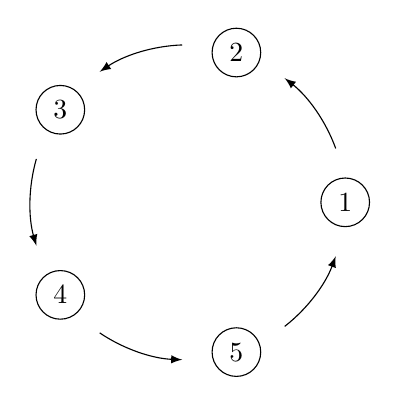
\begin{tikzpicture}

  \def \n {5}
  \def \radius {2cm}
  \def \margin {20} % margin in angles, depends on the radius

  \foreach \s in {1,...,\n} {
    \node[draw, circle] at ({360/\n * (\s - 1)}:\radius) {\(\s\)};
    \draw[->, >=latex] ({360/\n * (\s - 1)+\margin}:\radius)
      arc ({360/\n * (\s - 1)+\margin}:{360/\n * (\s)-\margin}:\radius);
  }
  \end{tikzpicture}
\end{center}

\bigskip

\textbf{Exercise 3.8}

\bigskip

\textbf{Solution}

Condensation method for the left-hand sided matrix is that
\[
\begin{split}
  \matxxxxx{2 & -1 & 2 & 1 & -3}{1 & 2 & 1 & -1 & 2}{1 & -1 & -2 & -1 & -1}{2 & 1 & -1 & -2 & -1}{1 & -2 & -1 & -1 & 2} \\
  & = \matxxxx
  {
    \matxx{2 & -1}{1 & 2} &
    \matxx{-1 & 2}{2 & 1} &
    \matxx{2 & 1}{1 & -1} &
    \matxx{1 & -3}{-1 & 2}
  }
  {
    \matxx{1 & 2}{1 & -1} &
    \matxx{2 & 1}{-1 & -2} &
    \matxx{1 & -1}{-2 & -1} &
    \matxx{-1 & 2}{-1 & -1}
  }
  {
    \matxx{1 & -1}{2 & 1} &
    \matxx{-1 & -2}{1 & -1} &
    \matxx{-2 & -1}{-1 & -2} &
    \matxx{-1 & -1}{-2 & -1}
  }
  {
    \matxx{2 & 1}{1 & -2} &
    \matxx{1 & -1}{-2 & -1} &
    \matxx{-1 & -2}{-1 & -1} &
    \matxx{-2 & -1}{-1 & 2}
  } \\
  & = \matxxxx{5 & -5 & -3 & -1}{-3 & -3 & -3 & 3}{3 & 3 & 3 & -1}{-5 & -3 & -1 & -5} \\
  & = \matxxx
  {
    \matxx{5 & -5}{-3 & -3} &
    \matxx{-5 & -3}{-3 & -3} &
    \matxx{-3 & -1}{-3 & 3}
  }
  {
    \matxx{-3 & -3}{3 & 3} &
    \matxx{-3 & -3}{3 & 3} &
    \matxx{-3 & 3}{3 & -1}
  }
  {
    \matxx{3 & 3}{-5 & -3} &
    \matxx{3 & 3}{-3 & -1} &
    \matxx{3 & -1}{-1 & -5}
  } \\
  & = \matxxx{-15 & 6 & 12}{0 & \mathbf{0} & 6}{6 & -6 & 8}
\end{split}
\]

Condenstaion method for the right-sided matrix shows the steps

\[
  \begin{split}
    \matxxxxx
    {1 &  2 & 1 &  -1 &  2}
    {1 & -1 & -2 & -1 & -1}
    {2 &  1 & -1 & -2 & -1}
    {1 & -2 & -1 & -1 &  2}
    {2 & -1 &  2 &  1 & -3}
    & = \matxxxx
    {
      \matxx{1 & 2}{1 & -1} &
      \matxx{2 & 1}{-1 & -2} &
      \matxx{1 & -1}{-2 & -1} &
      \matxx{-1 & 2}{-1 & -1}
    }
    {
      \matxx{1 & -1}{2 & 1} &
      \matxx{-1 & -2}{1 & -1} &
      \matxx{-2 & -1}{-1 & -2} &
      \matxx{-1 & -1}{-2 & -1}
    }
    {
      \matxx{2 & 1}{1 & -2} &
      \matxx{1 & -1}{-2 & -1} &
      \matxx{-1 & -2}{-1 & -1} &
      \matxx{-2 & -1}{-1 & 2}
    }
    {
      \matxx{1 & -2}{2 & -1} &
      \matxx{-2 & -1}{-1 & 2} &
      \matxx{-1 & -1}{2 & 1} &
      \matxx{-1 & 2}{1 & -3}
    } \\
    & = \matxxxx
    {-3 & -3 & -3 &  3}
    {3 &  3 &  3 & -1}
    {-5 & -3 & -1 & -5}
    {3 & -5 &  1 &  1} \\
    & = \matxxx
    {
      \matxx{-3 & -3}{3 & 3} &
      \matxx{-3 & -3}{3 & 3} &
      \matxx{-3 & 3}{3 & -1}
    }
    {
      \matxx{3 & 3}{-5 & -3} &
      \matxx{3 & 3}{-3 & -1} &
      \matxx{3 & -1}{-1 & -5}
    }
    {
      \matxx{-5 & -3}{3 & -5} &
      \matxx{-3 & -1}{-5 & 1} &
      \matxx{-1 & -5}{1 & 1}
    } \\
    & = \matxxx{0 & 0 & 6}{6 & -6 & 8}{-17 & 7 & -4}
  \end{split}
\]

\pagebreak

\section{Reflection over the group project}

We, three of us, Yong Hoon Do, Chan Yang Yim and Dongwook Kim had a meeting every Friday from the second week of the quarter to do our first project. Before we jumped working on the first project, we google-searched about a determinant first to sense what context this paper is on. After that, we looked through the paper to solve the exercises. Usually, I and Chanyang typed up the paper and Dongwook gave solutions to us in his hand writing. Then, I and Chanyang checked the validation of his answers, and triple checked to write the answer up using Latex. This way made us fully understood how the computation works for each exercises and it finally led us not to have a mistake on every exercises.

In terms of languages during our collaborative works, we always strived to use the proper language to tackle something that really did not stand out. In particular, we recognized that the terminology of a minor is not really a minor for my education, but this is the determinant of the square matrix formed by deleting one row and one column from some larger square matrix. The use of mathematical language is getting familiar as the number of meetings increases, and we successfully completed the project.

Since the paper introduces two methods for calculating determinants,
we were interested in the algorithm how the Dodgson's condensation method works.
Meanwhile we were fascinated by its great method, we figured out how Laplace expansion works.

If I have a coefficient matrix \(2 \times 2\), we can build a system of linear equations with a zero vector constant \(\)
so that we may solve this system
\[
  \matxx{a & b & 0}{c & d & 0}
  \arrow{}
  \begin{matrix}
    ax + by = 0 \\
    cx + dy = 0
  \end{matrix}
\]

Now, we end up with
\[
  \begin{split}
    (da - bc)y  & = 0 \\
    da - bc & = 0 \hspace{0.5cm} \mbox{ if } y \neq 0
  \end{split}
\]

\noindent This is really a determinant for any matrix \(2 \times 2\), and this is the only solution
for that system of linear equations. Our investigation would apply to any other matrix \(n \times n\), and we finally found the pattern:
a number of terms for solving determinants of a matrix \(n \times n\) is as many as \(\mathbf{!n}\). Thus, a number of terms for a determinant of a matrix \(4 \times 4\) is \(\mathbf{24}\).

\bigskip

\noindent Even though we spent some time to figure out why Dodgson's condensation method works,
we didn't discover many clues, but we understood how it works. We now know that
Dodgson's condensation method is useuful when computing larger matrices \(n \times n\), but
every centered value for each term must not be zero to go to the next step. We checked and understood switching rows would be a way to
figure the problem out.

\bigskip

\noindent Overall, this paper critically helped a lot for us to understand how to compute determinants, and
also we learned how to discover minors and their complements in any matrices \(n \times n\).

\pagebreak

\section{Summary for Proof Paper}

After reading the proof paper, we understood why Dodgson's method is labeled as \textbf{Condensation}.
This is because his method recursively makes the square matrix as far as \(2 \times 2\), and finally get
the determinant for the original matrix \(n \times n\). At the first glance, the method looked really awesome as it really gives a
determinant, and this fact gave the motivation to us dig into the method. In particular, we tried to understand why dividing the most overlapped value is required as a necessary step when
condensing the matrix into the smaller \((n-1) \times (n-1)\) matrix since we noticed that this value must not be \(0\). Otherwise,
we would see an infinite value as the paper tells. We kept tracking why dividing really matters in order for getting the determinant.
While noticing this important notion for determining the determinant, the paper introduced how getting determinant can still be achieved as a solution by the case where facing a zero for dividing value: swapping rows.
We even take the advantage of \textit{cyclical transposition} since the most of the terms in the newly ordered-blocks will have been computed already and we only need to copy them.
We didn't fully understand why this really works, but we discovered that there would be the following fact based on this information:
the same determinant could be found from the different row-ordered matrices.

\[
  \begin{split}
    A & = \matxxx{7 & 8 & 9}{4 & 5 & 6}{1 & 3 & 3} \hspace{1.0cm} B = \matxxx{1 & 3 & 3}{7 & 8 & 9}{4 & 5 & 6} \\
  \end{split}
\]

\[
  \mbox{det}(A) = -6 = \mbox{det}(B)
\]

we are briefly understanding why these two matrices are giving the same determinant, but we are not sure how to give a full proof yet.
This may be left as an additional topic for us to dig into later when we have a spare time. Overall, we wholeheartedly enjoyed reading the paper
about computing the determinants.

\end{document}
